\documentclass{book}

% ======== Packages ========
\usepackage[a4paper, top=2cm, bottom=3cm, left=2.5cm, right=2.5cm]{geometry}
\usepackage{titlesec}
\usepackage{fancyhdr}
\usepackage{amsmath}
\usepackage{graphicx} % buat gambar
\usepackage{pagecolor} % buat warna background
\usepackage{multicol}
\usepackage{amsfonts}
\usepackage{amssymb}
\usepackage{tikz}
\usepackage{array}
\usepackage{xcolor}
\usepackage{etoolbox}
\usepackage[hidelinks]{hyperref}
\usepackage{lipsum}
\usepackage{lettrine}
\usepackage{listings}
\usepackage{inconsolata}
\usetikzlibrary{positioning, arrows.meta, shapes.geometric}

% ======== Custom Drop Cap Font (Zallman) ========
\usepackage{filecontents}
\begin{filecontents*}{Zallman.sty}
  \NeedsTeXFormat{LaTeX2e}
  \ProvidesPackage{Zallman}[2007/11/24 v1.0 Zallman CFR]
  \input Zallman.fd
  \DeclareRobustCommand{\Zallmanfamily}{
    \fontencoding{U}%
    \fontseries{xl}%
    \fontshape{n}%
    \fontfamily{Zallman}%
    \selectfont}
  \DeclareTextFontCommand{\zall}{\Zallmanfamily}
  \endinput
\end{filecontents*}
\usepackage{Zallman}
\renewcommand{\LettrineFontHook}{\color{Maroon}\Zallmanfamily}

% ======== Colors ========
\definecolor{deepred}{RGB}{153, 0, 0}
\definecolor{codebg}{RGB}{240,240,240}
\definecolor{codeborder}{RGB}{200,200,200}
\definecolor{keywordcolor}{RGB}{153, 0, 0}
\definecolor{Maroon}{RGB}{128, 0, 0}

% ======== Code Style ========
\lstdefinestyle{mystyle}{
  backgroundcolor=\color{codebg},
  basicstyle=\ttfamily\footnotesize,
  frame=single,
  rulecolor=\color{codeborder},
  keywordstyle=\color{keywordcolor}\bfseries,
  commentstyle=\color{gray},
  stringstyle=\color{blue},
  showstringspaces=false,
  breaklines=true,
  language=Python
}

% ======== Chapter spacing tweak ========
\makeatletter
\patchcmd{\@makechapterhead}{\vspace*{50\p@}}{\vspace*{10pt}}{}{}
\makeatother

\usepackage{fancyhdr}
\pagestyle{fancy}
\fancyhf{} 
\fancyfoot[L]{\small\textit{Deep Thinking, made with \LaTeX{}}}
\fancyfoot[R]{\small Fauzy, This book only for learning purpose only \textbar\ 2025}
\renewcommand{\footrulewidth}{0.4pt}
\renewcommand{\headrulewidth}{0pt}


% ======== Chapter style ========
\titleformat{\chapter}[display]
  {\normalfont\Large\bfseries}
  {\begin{tikzpicture}
      \fill[deepred] (0,0) rectangle (2,-2.8);
      \node[text=white, font=\small\bfseries, anchor=base] at (1,-0.3) {CHAPTER};
      \node[text=white, font=\fontsize{30}{36}\selectfont\bfseries] at (1,-1.5) {\thechapter};
    \end{tikzpicture}}
  {0.5em}
  {\MakeUppercase}
  [\vspace{0.3em}
   \small\itshape\mdseries\raggedleft
   "The true logic of this world is in the calculus of probabilities." \\
   \rule{\linewidth}{0.4pt} \\
   \textbf{--- James C. Maxwell}]
\titlespacing*{\chapter}{0pt}{0pt}{2em}

\titleformat{\section}
  {\normalfont\bfseries}
  {\thesection}
  {1em}{}

\titleformat{\subsection}
  {\normalfont\bfseries}
  {\thesubsection}
  {1em}{}

\newcolumntype{L}[1]{>{\raggedright\arraybackslash}p{#1}}
\newcolumntype{R}[1]{>{\raggedleft\arraybackslash}p{#1}}

% ======== Document starts ========
\begin{document}

% === COVER PAGE ===
\begin{titlepage}
\centering
\vspace*{3cm}
{\Huge\bfseries DEEP THINKING\par}
\vspace{0.5cm}
{\Large\itshape Notes on Learning Machines and the Human Mind\par}
\vspace{2cm}
{\LARGE\scshape Fauzy Madani\par}
\vfill
{\Large SMK Negeri 1 Garut \\ \texttt{fauzy\_madani@smknegeri1garut.sch.id}}
\vspace*{2cm}
\end{titlepage}

% === Author Page ===
\chapter*{About the Author}
\addcontentsline{toc}{chapter}{About the Author}

\vspace{2em}

\newcommand{\HRule}{\rule{\linewidth}{0.5mm}}

\begin{center}
  \textsc{\LARGE SMKN 1 Garut}\\[1.5cm] % Institution / school
  
  \textsc{\Large Cloud Computing and Web Development Enthusiast}\\[0.5cm] % Major heading
  
  \textsc{\large About the Author}\\[0.5cm] % Minor heading (optional)
  
  \HRule\\[0.4cm]
  
  {\huge\bfseries Fauzy Madani}\\[0.4cm] % Large name
  
  \HRule\\[1.5cm]
\end{center}

\noindent
\begin{minipage}{0.48\textwidth}
  \large
  \textit{Contact}\\
  \texttt{github.com/fauzymadani} \\
  \texttt{fauzy@example.com}
\end{minipage}
\hfill
\begin{minipage}{0.48\textwidth}
  \large
  \textit{Areas of Interest}\\
  \begin{itemize}
    \setlength\itemsep{0.6em}
    \item Linux and Open Source Systems
    \item Cloud Infrastructure (AWS, Debian-based servers)
    \item Programming (Python, Bash, PHP)
    \item Machine Learning and Data Science
    \item Internet Privacy and Cryptography
  \end{itemize}
\end{minipage}

\vfill

\begin{center}
  {\large \today} % date, you can replace with fixed date if you want
\end{center}

\vspace{2em}

\noindent Fauzy Madani is a student at SMKN 1 Garut, passionate about cloud computing and web development. He actively explores open-source systems, Linux server administration, and secure web development.

His interests also include the intersection of machine learning and human cognition, with experiments in neural networks and data visualization. Fauzy shares his projects on GitHub and participates in various technology competitions, including Cloud Computing contests (LKS).

His long-term goal is to become a Debian package maintainer and contribute to reliable, privacy-focused software for the global community.

\clearpage

% === Table of Contents ===
% === CHAPTER 1 ===
\tableofcontents
\clearpage

\chapter{How to Use This Book}

\noindent
\textbf{Preface:}  
Welcome! Whether you are a beginner eager to learn or an experienced reader looking to deepen your understanding, this book is built to adapt to your pace. Each chapter stands on its own yet connects to a bigger picture—encouraging exploration and discovery rather than a strict linear path.  
Use the table of contents to navigate, skip ahead, or revisit concepts anytime you want. Don't worry about reading every page front to back. Instead, dive into topics that spark your curiosity, experiment with the exercises, and reflect on the ideas presented.  
This approach will help you develop a thoughtful, flexible mindset that’s essential for tackling complex problems in technology, science, or any field where deep understanding matters.

% Illustration
\begin{center}
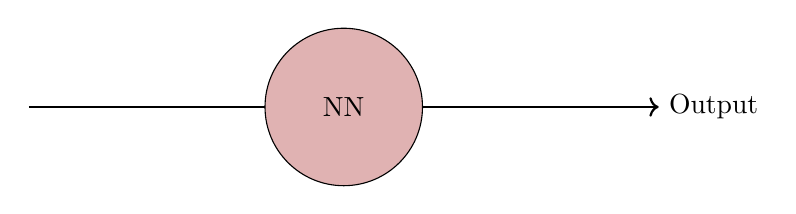
\begin{tikzpicture}
  \draw[->, thick] (0,0) -- (4,0) node[anchor=west] {Input};
  \draw[->, thick] (4,0) -- (8,0) node[anchor=west] {Output};
  \draw[fill=deepred!30] (4,0) circle (1);
  \node at (4,0) {NN};
\end{tikzpicture}

\vspace{0.5cm}
{\itshape Visual representation of a simple neural network.}
\end{center}

\section{Introduction}
\lettrine{T}{ he} field of neural networks represents a fundamental cornerstone of modern artificial intelligence. At its core, a neural network functions as a system that transforms input data into meaningful output through layers of interconnected nodes, mimicking certain aspects of human brain processing. This transformative process enables machines to learn patterns, recognize complex structures, and make informed decisions across a wide range of applications.
In this book, we explore the principles, architectures, and techniques that underlie neural networks and their broader implications in machine learning. Beyond the technical details, we emphasize a mindset of thoughtful analysis and deliberate problem-solving—key skills necessary to navigate the evolving landscape of AI and data science.

\subsection{What makes this book so valuable}
\lettrine{D}{ eciphering} dead languages. Detecting malignant tumours. develop a skill that’s crucial but often overlooked: the ability to analyze complex problems thoughtfully and thoroughly. In today’s fast-paced world, many people tend to skim information or jump to quick conclusions, but deep thinking encourages slowing down, questioning assumptions, and understanding systems at a fundamental level. Such a book would provide practical frameworks and mental tools to approach challenges more effectively, whether in everyday life, science, engineering, or technology. It can also bridge the gap between abstract reasoning and real-world application, helping readers not just to think harder but to think smarter—anticipating problems, designing better solutions, and making decisions that stand the test of time. Ultimately, its value lies in empowering readers to cultivate clarity, insight, and creativity, which are essential for innovation and meaningful progress in any field.
in an age where information flows rapidly and superficially, the ability to think deeply and critically is more important than ever. This book aims to cultivate that skill by providing readers with practical frameworks to approach complex problems with clarity and rigor. Whether you are decoding ancient languages, diagnosing medical conditions, or building intelligent systems, the methods discussed here foster a thorough understanding of underlying processes and encourage innovative solutions.
By bridging theoretical concepts with real-world applications, this work empowers readers to think not only harder but smarter—anticipating challenges, crafting robust designs, and making decisions grounded in insight and foresight. Ultimately, the goal is to nurture creativity and precision, equipping you with the tools needed for meaningful progress in any technical or scientific endeavor.

% === CHAPTER 2 ===
\chapter{Deep Learning Basics}

\section{What is a Neural Network?}
\lettrine{A}{ rtificial} type of computational model inspired by the way biological brains work, designed to recognize patterns and solve complex problems by learning from data. At its core, a neural network is composed of many interconnected units called neurons or nodes, arranged in layers. These layers typically include an input layer, one or more hidden layers, and an output layer.
Each neuron receives input signals (which are usually numbers) from neurons in the previous layer, processes them by applying a weighted sum followed by a non-linear function called an activation function, and then passes the result to neurons in the next layer. The weights represent the strength or importance of the connections, and the activation function introduces non-linearity, enabling the network to model complex relationships rather than just linear ones.
Training a neural network involves adjusting these weights so that the network’s output matches the desired output as closely as possible. This is done through a process called backpropagation combined with an optimization algorithm like gradient descent. Backpropagation works by calculating the error between the predicted output and the actual output, then propagating this error backward through the network to update the weights in a way that reduces the error over time.
Neural networks are particularly powerful because they can automatically learn representations from raw data without needing explicit feature engineering. For example, in image recognition, early layers might detect simple features like edges, while deeper layers identify more complex shapes or objects.
There are many types of neural networks designed for specific tasks. For instance, feedforward neural networks process data in one direction from input to output, while recurrent neural networks (RNNs) have loops allowing them to process sequences and remember past information, which is useful in language processing. Another type, convolutional neural networks (CNNs), uses specialized layers to efficiently analyze visual data.
Overall, neural networks form the backbone of many modern AI applications, including speech recognition, natural language processing, autonomous driving, and more, because of their ability to learn complex patterns and generalize well to new, unseen data.

\subsection{Perceptron}
\lettrine{T}{ he} perceptron is a binary classifier. perceptron is one of the simplest types of artificial neural networks and actually a foundational building block for more complex neural networks. It was introduced in the 1950s by Frank Rosenblatt.
A perceptron takes several input values, each multiplied by a weight that represents the importance of that input. Then, it sums all these weighted inputs and passes the result through an activation function, typically a step function that outputs either 0 or 1. This output represents the perceptron’s decision—like classifying data into one of two categories.
Mathematically, if you think of inputs as a vector xx and weights as ww, the perceptron computes:
$$ y = \text{activation}\left(\sum_{i=1}^n w_i x_i + b \right) $$
where bb is a bias term that shifts the decision boundary.
The perceptron learns by adjusting the weights based on errors between its predicted output and the actual target during training, using a simple update rule. While a single perceptron can only solve linearly separable problems (where a straight line can separate classes), stacking perceptrons and adding layers leads to more powerful models like multilayer neural networks that can learn complex patterns.
In short, the perceptron is the building block for neural networks, helping machines make simple yes/no decisions and forming the basis for deep learning architectures.

\section{Training the model}
\noindent
Training a model involves finding the right set of parameters (weights and biases) that minimize the error between the predicted output and the actual output. This process is essentially an optimization problem. The model "learns" by iteratively adjusting its parameters using algorithms like gradient descent. Over time, these adjustments improve the model's accuracy.
\begin{center}
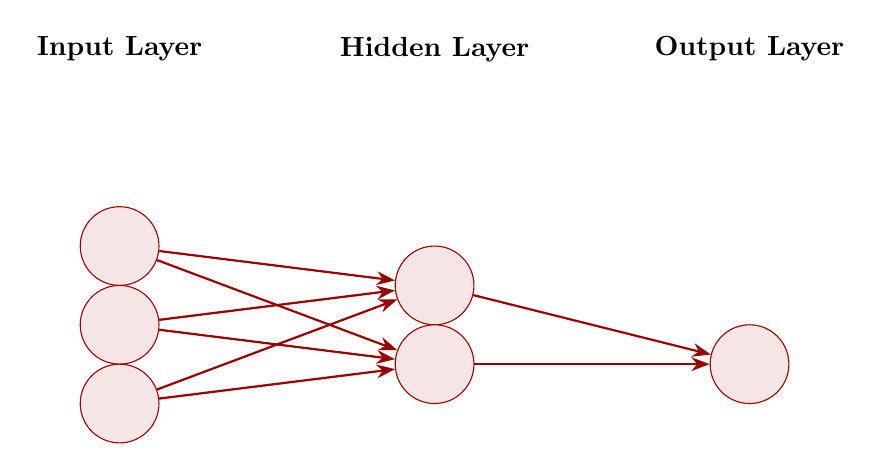
\begin{tikzpicture}[
  neuron/.style={circle, draw=deepred, fill=deepred!10, minimum size=1cm},
  layer/.style={draw=none, font=\bfseries},
  connection/.style={->, thick, >=Stealth, draw=deepred},
  node distance=1cm and 1.5cm
]
  % Layers
  \node[layer] at (0,3.5) {Input Layer};
  \node[layer] at (4,3.5) {Hidden Layer};
  \node[layer] at (8,3.5) {Output Layer};

  % Input neurons
  \foreach \i in {1,2,3} {
    \node[neuron] (i\i) at (0,2-\i) {};
  }

  % Hidden neurons
  \foreach \j in {1,2} {
    \node[neuron] (h\j) at (4,1.5-\j) {};
  }

  % Output neuron
  \node[neuron] (o1) at (8,-0.5) {};

  % Connections: Input -> Hidden
  \foreach \i in {1,2,3} {
    \foreach \j in {1,2} {
      \draw[connection] (i\i) -- (h\j);
    }
  }

  % Connections: Hidden -> Output
  \foreach \j in {1,2} {
    \draw[connection] (h\j) -- (o1);
  }
\end{tikzpicture}

\vspace{0.5em}
\textit{Figure: A basic neural network during training. Weights are updated to reduce prediction error.}
\end{center}

\subsection{Backpropagation}
\vspace{0.5em}
\noindent
To understand how errors propagate backward through layers, consider the basic gradient descent update rule:
\begin{equation}
  w := w - \eta \frac{\partial L}{\partial w}
\end{equation}

\noindent
Where:
\begin{itemize}
  \item \textit{\( w \)} is a weight parameter,
  \item \textit{\( \eta \)} is the learning rate,
  \item \textit{\( \frac{\partial L}{\partial w} \)} is the partial derivative of the loss function with respect to the weight.
\end{itemize}

\vspace{0.4em}
\begin{center}
  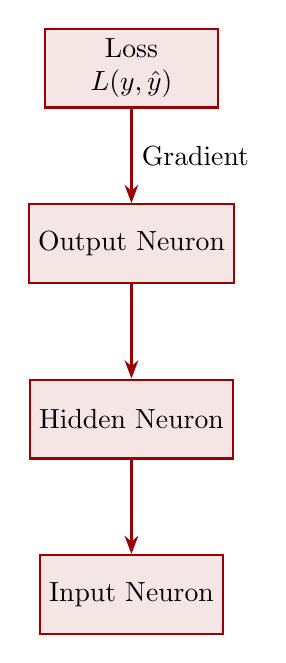
\begin{tikzpicture}[
    block/.style={
      rectangle,
      draw=deepred,
      thick,
      fill=deepred!10,
      minimum width=2.2cm,
      minimum height=1cm,
      align=center
    },
    arrow/.style={->, thick, >=Stealth, draw=deepred},
    node distance=1.2cm
  ]
    \node[block] (loss) {Loss \\ \( L(y, \hat{y}) \)};
    \node[block, below=of loss] (output) {Output Neuron};
    \node[block, below=of output] (hidden) {Hidden Neuron};
    \node[block, below=of hidden] (input) {Input Neuron};

    \draw[arrow] (loss) -- node[right] {Gradient} (output);
    \draw[arrow] (output) -- (hidden);
    \draw[arrow] (hidden) -- (input);
  \end{tikzpicture}

  \vspace{0.4em}
  \textit{Figure: Backpropagation through layers using gradient descent.}
\end{center}

\vspace{0.3em}
\noindent
Backpropagation efficiently applies the chain rule:
\begin{equation}
  \frac{\partial L}{\partial w} =
  \frac{\partial L}{\partial y} \cdot
  \frac{\partial y}{\partial z} \cdot
  \frac{\partial z}{\partial w}
\end{equation}

\noindent
Each term in this chain corresponds to a different layer in the network, enabling us to compute how much each weight contributes to the overall loss.

\lettrine{B}{ ackpropagation} is an essential technique. fundamental algorithm in AI and deep learning that enables neural networks to learn from data by adjusting their internal parameters—called weights—in order to improve performance on a given task. When a neural network processes an input, it produces an output, which is then compared to the expected or correct result using a loss function—a measure of how far off the prediction is. The goal of training is to minimize this loss.
Backpropagation works by computing the gradient, or the rate of change, of the loss function with respect to each weight in the network. This gradient tells us how much a small change in a particular weight will affect the overall error. The algorithm uses the chain rule from calculus to efficiently calculate these gradients layer by layer, starting from the output layer and moving backward toward the input layer—hence the name “backpropagation.”
Once the gradients are computed, they guide how the weights should be adjusted. Using an optimization method like gradient descent, the network updates its weights in the direction that most reduces the loss. This process repeats over many iterations (epochs), gradually improving the network’s accuracy in making predictions.
Without backpropagation, training deep neural networks would be extremely difficult because it allows the model to assign credit or blame to each connection based on its contribution to the final error, enabling the network to learn complex, multi-layered representations from data. This makes backpropagation a cornerstone technique that drives much of the progress in deep learning and modern AI applications.

% Complex Flowchart
\begin{center}
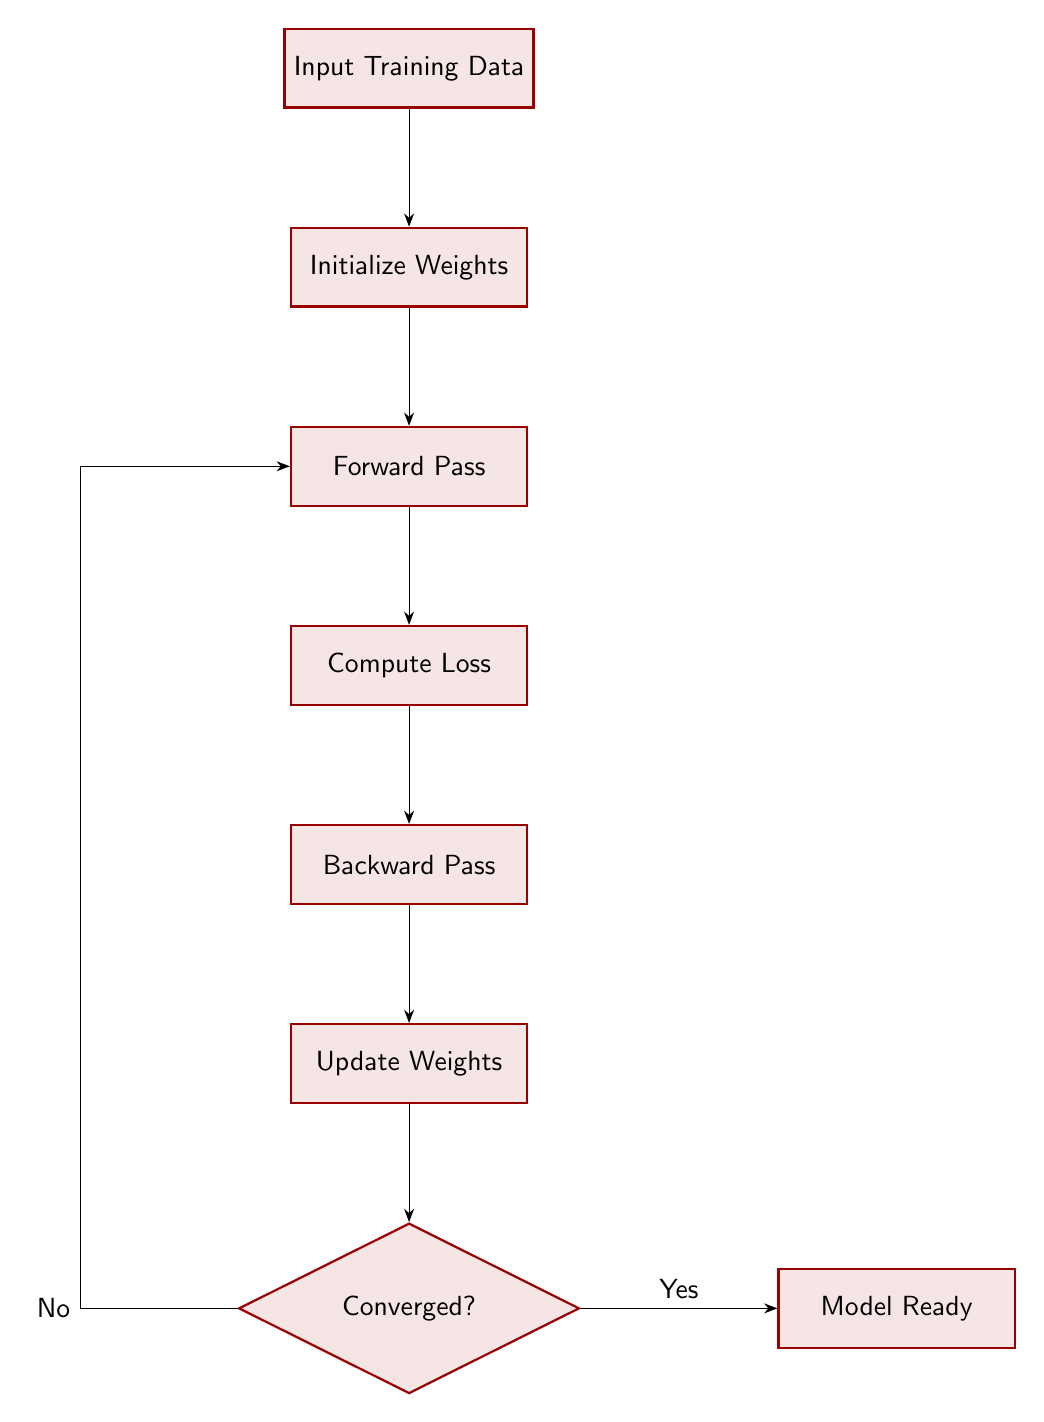
\begin{tikzpicture}[
  node distance=1.5cm and 2.5cm,
  every node/.style={font=\sffamily},
  process/.style={rectangle, draw=deepred, thick, fill=deepred!10, minimum width=3cm, minimum height=1cm},
  decision/.style={diamond, draw=deepred, thick, fill=deepred!10, aspect=2, text width=3cm, align=center},
  >=Stealth
]

\node[process] (data) {Input Training Data};
\node[process, below=of data] (init) {Initialize Weights};
\node[process, below=of init] (fwd) {Forward Pass};
\node[process, below=of fwd] (loss) {Compute Loss};
\node[process, below=of loss] (bwd) {Backward Pass};
\node[process, below=of bwd] (update) {Update Weights};
\node[decision, below=of update] (check) {Converged?};
\node[process, right=of check] (done) {Model Ready};

\draw[->] (data) -- (init);
\draw[->] (init) -- (fwd);
\draw[->] (fwd) -- (loss);
\draw[->] (loss) -- (bwd);
\draw[->] (bwd) -- (update);
\draw[->] (update) -- (check);
\draw[->] (check) -- node[above] {Yes} (done);
\draw[->] (check.west) -- ++(-2,0) node[left] {No} |- (fwd.west);

\end{tikzpicture}

\vspace{0.5cm}
{\itshape A more detailed training loop in a deep learning pipeline.}
\end{center}

\begin{lstlisting}[style=mystyle, caption={A simple neural net in PyTorch}]
import torch
import torch.nn as nn

class Net(nn.Module):
    def __init__(self):
        super(Net, self).__init__()
        self.fc = nn.Linear(10, 1)

    def forward(self, x):
        return self.fc(x)
\end{lstlisting}

% === CHAPTER 3 ===
% === CHAPTER 3 ===
\chapter{Advanced Topics}

\section{Generative Adversarial Networks (GANs) and Variational Autoencoders (VAEs)}

\lettrine{G}{enerative} models have revolutionized how machines can create data resembling real-world distributions. Two of the most influential models in this domain are Generative Adversarial Networks (GANs) and Variational Autoencoders (VAEs), each with a unique approach to data generation.

\vspace{0.5cm}
% Simple GAN architecture illustration
\begin{center}
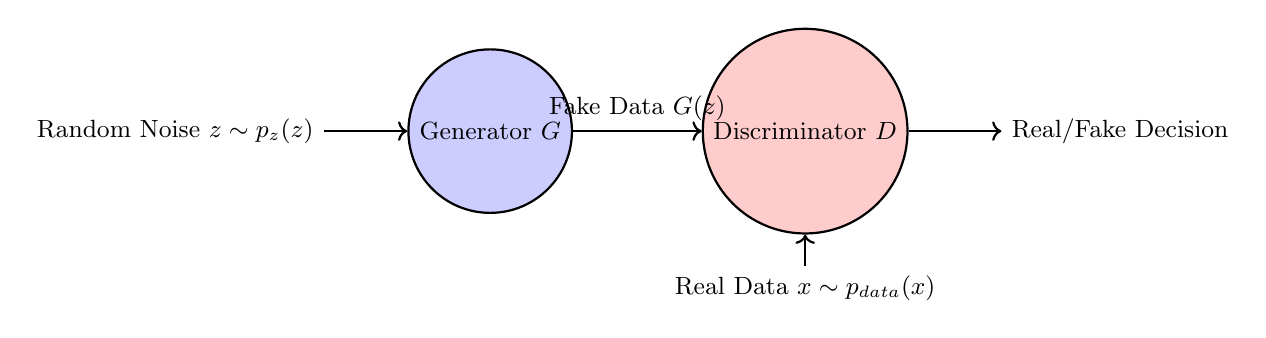
\begin{tikzpicture}[thick, every node/.style={font=\small}]
  % Nodes
  \node (noise) at (0,0) {Random Noise \( z \sim p_z(z) \)};
  \node[draw, circle, fill=blue!20, minimum size=1.2cm] (gen) at (4,0) {Generator \( G \)};
  \node[draw, circle, fill=red!20, minimum size=1.2cm] (disc) at (8,0) {Discriminator \( D \)};
  \node (realfake) at (12,0) {Real/Fake Decision};

  % Arrows
  \draw[->] (noise) -- (gen);
  \draw[->] (gen) -- (disc) node[midway, above] {Fake Data \( G(z) \)};
  \draw[->] (disc) -- (realfake);

  % Real data arrow
  \node (real) at (8,-2) {Real Data \( x \sim p_{data}(x) \)};
  \draw[->] (real) -- (disc);
\end{tikzpicture}
\end{center}

\vspace{0.5cm}
GANs consist of two neural networks — a Generator \(G\) that synthesizes data from random noise \(z\), and a Discriminator \(D\) that evaluates whether the data is real or fake. Both networks engage in a minimax game defined by the value function:

\[
\min_G \max_D V(D, G) = \mathbb{E}_{x \sim p_{data}(x)}[\log D(x)] + \mathbb{E}_{z \sim p_z(z)}[\log(1 - D(G(z)))]
\]

where \(p_{data}\) is the true data distribution, and \(p_z\) is the noise prior.

\vspace{0.5cm}
In contrast, VAEs approach generative modeling by learning a probabilistic mapping between data and a latent space. VAEs optimize the evidence lower bound (ELBO):

\[
\mathcal{L}(\theta, \phi; x) = \mathbb{E}_{q_\phi(z|x)}[\log p_\theta(x|z)] - D_{KL}(q_\phi(z|x) \| p(z))
\]

where \(q_\phi(z|x)\) is the encoder’s approximate posterior, \(p_\theta(x|z)\) is the decoder likelihood, and \(D_{KL}\) is the Kullback-Leibler divergence ensuring the latent distribution stays close to prior \(p(z)\), typically Gaussian.

\vspace{0.5cm}
% VAE graphical illustration
\begin{center}
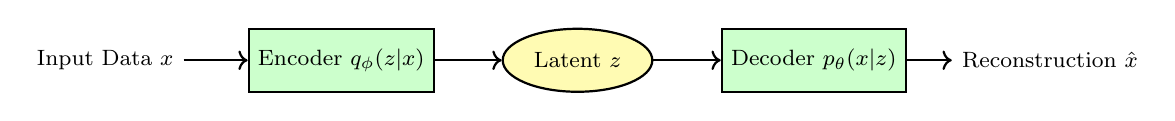
\begin{tikzpicture}[thick, every node/.style={font=\footnotesize}]  % font sedikit lebih kecil
  % Nodes
  \node (input) at (0,0) {Input Data \( x \)};
  \node[draw, rectangle, fill=green!20, minimum width=1.5cm, minimum height=0.8cm] (encoder) at (3,0) {Encoder \( q_\phi(z|x) \)};
  \node[draw, ellipse, fill=yellow!30, minimum width=1.2cm, minimum height=0.8cm] (latent) at (6,0) {Latent \( z \)};
  \node[draw, rectangle, fill=green!20, minimum width=1.5cm, minimum height=0.8cm] (decoder) at (9,0) {Decoder \( p_\theta(x|z) \)};
  \node (recon) at (12,0) {Reconstruction \( \hat{x} \)};

  % Arrows
  \draw[->] (input) -- (encoder);
  \draw[->] (encoder) -- (latent);
  \draw[->] (latent) -- (decoder);
  \draw[->] (decoder) -- (recon);
\end{tikzpicture}
\end{center}

\vspace{0.5cm}
Both GANs and VAEs have proven to be powerful generative models with complementary strengths: GANs excel at producing sharp, realistic samples by learning through adversarial competition, whereas VAEs provide a principled probabilistic framework allowing smooth latent space interpolation and meaningful data representations.

\vspace{0.3cm}
Understanding these models opens pathways to advanced applications including image synthesis, anomaly detection, data augmentation, and creative AI.

% === CHAPTER 4 ===
\chapter{Interview Questions}

\section{Theory}
\lettrine{T}{heory} questions in interviews often test your understanding of key deep learning concepts:

\begin{itemize}
  \item \textbf{Backpropagation}: uses chain rule to compute gradients.
  \item \textbf{Activation Functions}: like ReLU and sigmoid help networks learn non-linear patterns.
  \item \textbf{GANs}: involve two networks (generator and discriminator) competing in a minimax game.
  \item \textbf{VAEs}: combine autoencoders with probabilistic inference.
\end{itemize}

deep learning models combines ideas from mathematics and computer science: neural networks approximate complex functions by layering simple mathematical operations, and backpropagation uses calculus to efficiently adjust the network’s parameters to reduce errors. GANs rely on game theory, where two networks compete to generate realistic data by learning the true data distribution, while VAEs use principles from probability and Bayesian inference to learn compact, meaningful representations of data and generate new samples by balancing reconstruction accuracy with keeping the underlying data structure organized. Together, these theories enable machines to learn from data, recognize patterns, and create new content in powerful and flexible ways.

\vspace{0.3cm}
\noindent\textbf{Backprop Formula}:
\[
\frac{\partial \mathcal{L}}{\partial w} = \frac{\partial \mathcal{L}}{\partial a} \cdot \frac{\partial a}{\partial z} \cdot \frac{\partial z}{\partial w}
\]

\vspace{0.4cm}
\begin{center}
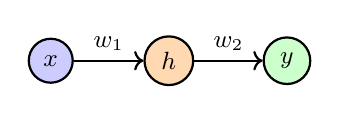
\begin{tikzpicture}[node distance=1.5cm, thick, every node/.style={font=\small}]
  \node (x) [draw, circle, fill=blue!20] {\(x\)};
  \node (h) [right of=x, draw, circle, fill=orange!30] {\(h\)};
  \node (y) [right of=h, draw, circle, fill=green!20] {\(y\)};
  \draw[->] (x) -- (h) node[midway, above] {\(w_1\)};
  \draw[->] (h) -- (y) node[midway, above] {\(w_2\)};
\end{tikzpicture}

\smallskip
\textit{Simple neural network: input–hidden–output}
\end{center}

---

\section{Coding}

\lettrine{I}{nterviewers} often ask you to write code. t’s their goal is to assess more than just whether you
can produce a working program. They want to see your problem-solving process, logical thinking,
and how you approach complex challenges step-by-step—which is essentially a form of deep thinking
applied in a practical context. Writing code live reveals how you break down problems, choose the right
algorithms or data structures, and handle edge cases or errors. It also shows your ability to communicate
your reasoning clearly and adapt when faced with unfamiliar scenarios. So, the coding task isn’t just
about getting the right answer; it’s about demonstrating your mindset, technical skills, and capacity to
think deeply and logically under pressure, which are critical traits for real-world software development. 
test your logic and clarity when coding. Focus on correctness and clean thinking.

\vspace{0.4cm}
\noindent\textbf{Example: Reverse a String in Python}
\begin{verbatim}
def reverse_string(s):
    return s[::-1]
\end{verbatim}

\vspace{0.4cm}
\noindent\textbf{Tips:}
\begin{itemize}
  \item Think aloud while coding.
  \item Handle edge cases (empty input, null values).
  \item Use clear variable names and structure.
\end{itemize}

---

\chapter{Conclusion}
\begin{multicols}{2}

\section*{Overview}
\addcontentsline{toc}{section}{Overview}
\lettrine{T}{ his} book has explored a wide range of concepts in deep learning, from foundational theories to advanced architectures such as GANs and VAEs. Through theoretical explanation, visual illustrations, and code-driven insights, we have aimed to provide not just knowledge—but understanding. As the field of artificial intelligence continues to evolve rapidly, having a strong conceptual grasp is more valuable than ever before.

\section*{Key Takeaways}
\addcontentsline{toc}{section}{Key Takeaways}
\begin{itemize}
  \item Deep learning models approximate complex functions via layered transformations.
  \item GANs rely on adversarial training while VAEs use probabilistic modeling.
  \item Mathematical foundations like linear algebra, probability, and calculus are essential.
  \item Real-world applications require both theoretical understanding and coding fluency.
  \item Thinking deeply—not just quickly—results in better solutions and more robust systems.
\end{itemize}

\section*{Reflection on Deep Thinking}
\addcontentsline{toc}{section}{Reflection on Deep Thinking}
Deep thinking is not about overcomplicating ideas. It’s about stripping concepts down to their essence and building back up with clarity and intent. Throughout this book, we’ve highlighted the importance of pausing to truly understand: Why does a model work? What assumptions are baked into our algorithms? How can we design systems that are both intelligent and interpretable?

This reflection is not just academic—it’s practical. Engineers who deeply understand their tools are better equipped to improve them, debug them, and innovate beyond them.

\section*{Future Outlook}
\addcontentsline{toc}{section}{Future Outlook}
Artificial Intelligence is progressing at an exponential rate. In the coming years, we’ll likely see breakthroughs in:

\begin{itemize}
  \item Self-supervised and few-shot learning
  \item Explainable AI (XAI) and ethical frameworks
  \item Fusion between symbolic reasoning and deep neural architectures
  \item Lightweight and edge-deployable neural models
\end{itemize}

To prepare for these developments, it is crucial to remain both curious and rigorous. The mindset cultivated in this book—an analytical, structured, and reflective way of thinking—will serve as your strongest asset.

\section*{Final Words}
\addcontentsline{toc}{section}{Final Words}
Whether you are a student, researcher, engineer, or just an enthusiast, remember that deep learning is not only about machines learning from data—it’s also about humans learning from thinking. May your journey ahead be filled with discovery, creativity, and meaningful progress.

\end{multicols}

\cleardoublepage
\thispagestyle{empty}
\begin{center}
\vspace*{4cm}

{\Huge \bfseries Thank You for Reading}

\vspace{1.5cm}

{\Large Deep thinking is a skill, not just a mindset.}

\vspace{1.5cm}

\begin{center}
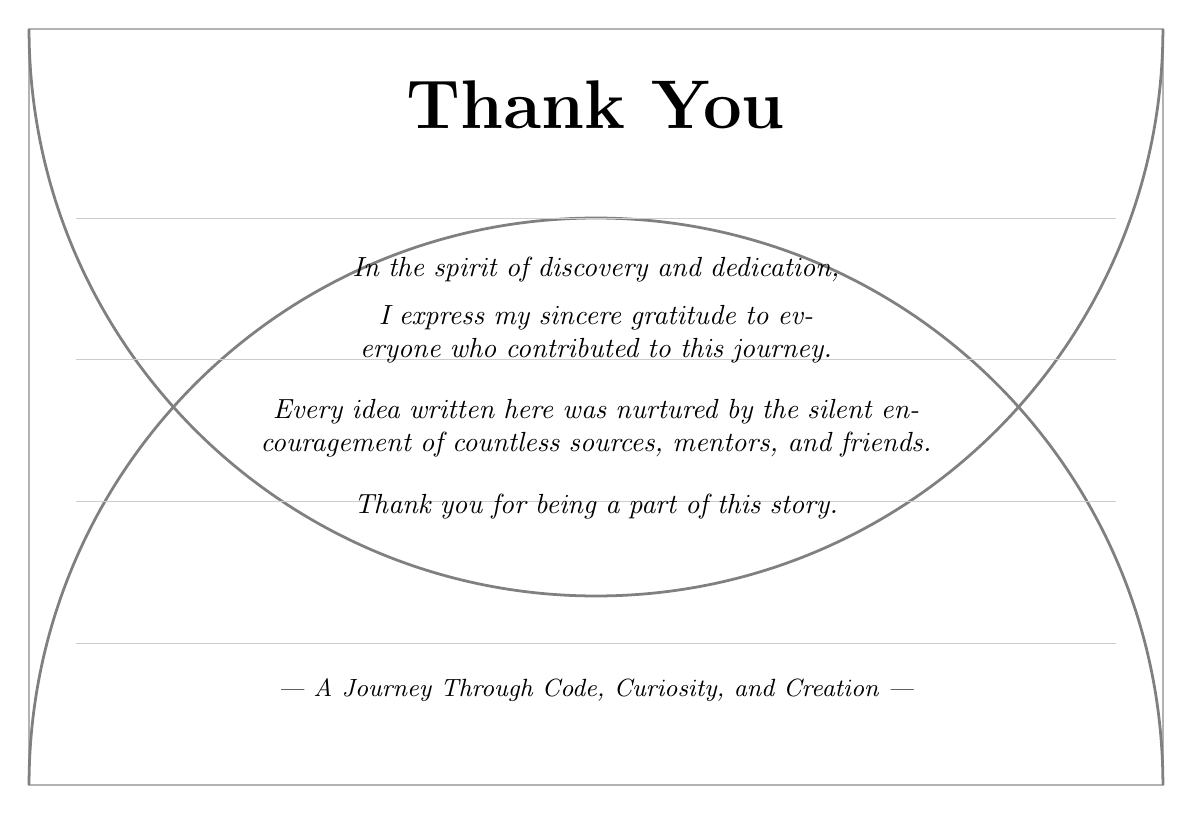
\begin{tikzpicture}[scale=1.2]

  % Frame
  \draw[line width=0.8pt, color=gray!60] (-6,0) rectangle (6,8);

  % Top curve
  \draw[line width=1pt, color=gray] (-6,8) arc[start angle=180,end angle=360,radius=6];

  % Bottom curve (mirrored)
  \draw[line width=1pt, color=gray] (6,0) arc[start angle=0,end angle=180,radius=6];

  % Decorative lines
  \foreach \y in {1.5,3,...,6.5}
    \draw[line width=0.2pt, color=gray!40] (-5.5,\y) -- (5.5,\y);

  % Main Title
  \node at (0,7.2) {\Huge\bfseries Thank You};

  % Message
  \node[align=center, text width=10cm] at (0,4.2) {\itshape
    In the spirit of discovery and dedication,\\[0.5em]
    I express my sincere gratitude to everyone who contributed to this journey.\\[1em]
    Every idea written here was nurtured by the silent encouragement of countless sources, mentors, and friends.\\[1em]
    Thank you for being a part of this story.
  };

  % Footer
  \node[align=center] at (0,1) {\small\itshape
    --- A Journey Through Code, Curiosity, and Creation ---};

\end{tikzpicture}
\end{center}

\vfill

{\large\itshape
May this book ignite not only your knowledge, but your curiosity.\\
Stay sharp. Keep building. Keep thinking deeply.
}

\vspace{3cm}

{\Large \textcopyright{} \the\year{} \ Fauzy Madani}

\end{center}

\cleardoublepage
\thispagestyle{empty}

\vspace*{3cm}
\begin{center}
    {\Huge\bfseries Acknowledgments}
\end{center}

\vspace{1cm}

\begin{multicols}{2}
\lettrine[lines=3,lhang=0.2,lraise=0.1]{T}{ hank} you for taking the time to read this work. This book was created primarily as a personal learning journey to master the art of \LaTeX\ and deepen my understanding of advanced topics in machine learning. 

The path of learning is endless, and I hope this effort not only strengthens my own skills but also inspires others who are passionate about technical writing and scientific exploration. 

Each page here is a step towards clarity, precision, and creativity — qualities essential both in academia and professional life. Like the intricate tales woven in classic literature, such as those found in the world of Harry Potter, knowledge too is a magic waiting to be discovered and shared.

By blending formality with imagination, this work strives to balance the rigor of scientific papers and the timeless charm of storytelling. I appreciate your interest and encourage you to keep questioning, experimenting, and creating.

May your own learning journey be as rewarding and magical as the worlds we build with words and equations.
\end{multicols}

\vspace{2cm}
\begin{center}
        \textit{— Fauzy, made with \LaTeX{}}
\end{center}

\end{document}

